Before diving into the architectural details of the system, we first present a state of the art summary, that concisely describes what is the positioning of this project in light of the previous explored \glspl{sna} tools that we presented in chapter 4, and also considering the \glspl{osn} that we study in chapter 3.\\
\indent Specifically regarding the \glspl{sna} tools, we will comment some of them, some of their useful features and overall comments to what may lack on this tools that this project may target, in order to differentiate and not only \textit{''reinvent the wheel''}.

\section{Simplicity}
Aside of \textbf{Vizster} (\cite{heer2005vizster}), the majority of the previously presented tools such as Gephi \cite{bastian2009gephi} or Social Network Visualizer \cite{socnetv}, are very complex tools with very heavy interfaces, that have a big learning and are meant for users that have particular advanced knowledge in \glspl{sn} and \glspl{sna}. The tool to be developed could also serve for less expert users, providing a set of core basic functionalities (e.g only allow users to load and visualize they're networks), and then, allow the user to build complexity from there enabling and disabling other features.

\section{Accessibility}
All the software that we presented above exists in the form of desktop applications. This applications need to be downloaded, and installed in a compatible machines (sometimes with dependencies on other software that is not installed by default). Nowadays almost every application is web based, this allows users to access them every where through a browser, making web apps a solution that is Operating System and device agnostic. This said, building a web based social networks analysis tool could be a way of tackle the accessibility of such tools.\\
\indent A web based application, it's good for sake of accessibility but in another hand it is a performance culprit when it comes to performance. This is a decision to take into account, but always having in mind that tackling performance it's not the main goal this master's thesis, also, the mentioned tools are mature projects that are highly performant and are capable of rendering huge networks.

\section{\acrfull{osn} integration}
Social Network Visualizer \cite{socnetv}, allows to \textit{scrap} web sites to build networks, but for this feature relies only on links to build the network (it blindly scraps recursively some url to build the network). By allowing the user to analyze networks that are directly reporting they're social network status would be a differentiation factor from the other tools, and would certainly be a more meaningful and valuable analysis for the end user.

\section{Drawing Accurate Conclusions}
As we state before when talking about simplicity, the mentioned \glspl{sna} tools provide generic metrics on networks such as network density or actor centrality. The values outputted from this tools are the result of running generic formulas and algorithms against some networks, so its very common for current \glspl{sna} researchers to be worried about the size of the network, being their focus on \textbf{quantitive analysis}.\\
\indent In a hypothetical analysis scenario where some researcher has a network with a few thousand nodes, \textbf{what is the meaning of his assumptions when analyzing the network}? Since this is a pure quantitive analysis the numbers will seem reasonable for the given network, but this will not allow him to extract contextual conclusions, because in this case analyzing data from Facebook or analyzing data from LinkedIn will sound just like the same, it would all comes down to the network. A better approach for drawing conclusions would be to have a mixture between \textbf{quantitive analysis} and \textbf{quality analysis}, the tool could do some content and context analysis, to help the end user on achieving more meaningful conclusions, rather than just some numerical metrics.

\section{System positioning and tools comparison}
In this section we will make a high level comparison between the software tools presented in chapter 4. In Table \ref{table:toolscompare} we can observe the tools classification based on some predefined metrics that show the positioning of the proposed system, these metrics are:

\begin{itemize}
    \item \textbf{Availability (Desktop or Web)} - Whether the tool available through a desktop application or a web application;
    \item \textbf{Complexity (Low, Moderate, High)} - Whether the tool has very complex features that require expertise to be used, also we may consider the learning curve for using the tool with efficiency;
    \item \textbf{Performance (Low, Medium , High)} - Whether the tool is performant, if it computes metrics with velocity and if it renders dense graphs without struggle;
    \item \textbf{Network Edition (Yes, No)} - Whether the tool allows network editing, such feature allows adding nodes and edges to existing network or event creating new networks from scratch;
    \item \textbf{\glspl{osn} Integration (Yes, No)} - Whether the tool is able to integrate data analysis of \glspl{osn}.
    \item \textbf{Contextual Analysis (Yes, No)} - By contextual analysis we do not mean that the user will not be aware of the network context, our contextual analysis has a strong meaning, it represents the capacity that the system demonstrates (or not) to be aware of the context of the network and providing metrics with a specific meaning.
\end{itemize}

\begin{table}[H]
\hspace*{-0.9in}
\renewcommand{\tabcolsep}{2pt}
\begin{tabular}{ |c|c|c|c|c|c|c|c|  }
\hline
\textbf{Tool} & \textbf{Availability} & \textbf{Complexity} & \textbf{Performance} & \textbf{Network Edition} & \textbf{\glspl{osn} Integration} & \textbf{Contextual Analysis}\\
\hline
\textbf{Structure} & Desktop & Moderate & Medium & Yes & No & No\\
\hline
\textbf{Gephi} & Desktop & Moderate & Good & Yes & No & No\\
\hline
\textbf{UCINET} & Desktop & High & Very Good & Yes & No & No\\
\hline
\textbf{SocNetV} & Desktop & Low & Medium & Yes & No\footnote{SocNetV has a feature that allows the user to launch a \textit{web spider} that navigates through web sites building a network representative of the links between the sites, but the \textit{spider} is not content aware, it blindly builds a network without context} & No\\
\hline
\textbf{\begin{tabular}{@{}c@{}}Our system\\projections\end{tabular}} & Web & Low & Low & No & Yes & Yes\\
\hline
\end{tabular}
\caption{\label{table:toolscompare} Software tools comparison and our system positioning.}
\end{table}

As we can observe in Table \ref{table:toolscompare} our system has essentially three differential factors, that are: web availability; \glspl{osn} integration; contextual analysis; being the trade off for such gains the system performance. When describing our system compared to the other tools we want to be able to have a web tool that has a complexity level similar to SocNetV.

\section{System Architecture}

Now, after building up our aiming for this project, we now present a more concrete image of the overall system. In Figure \ref{img:architectureprop} we present an abstract system architecture.

\begin{figure}[h!]
\begin{center}
  \hspace*{-0.8in}
  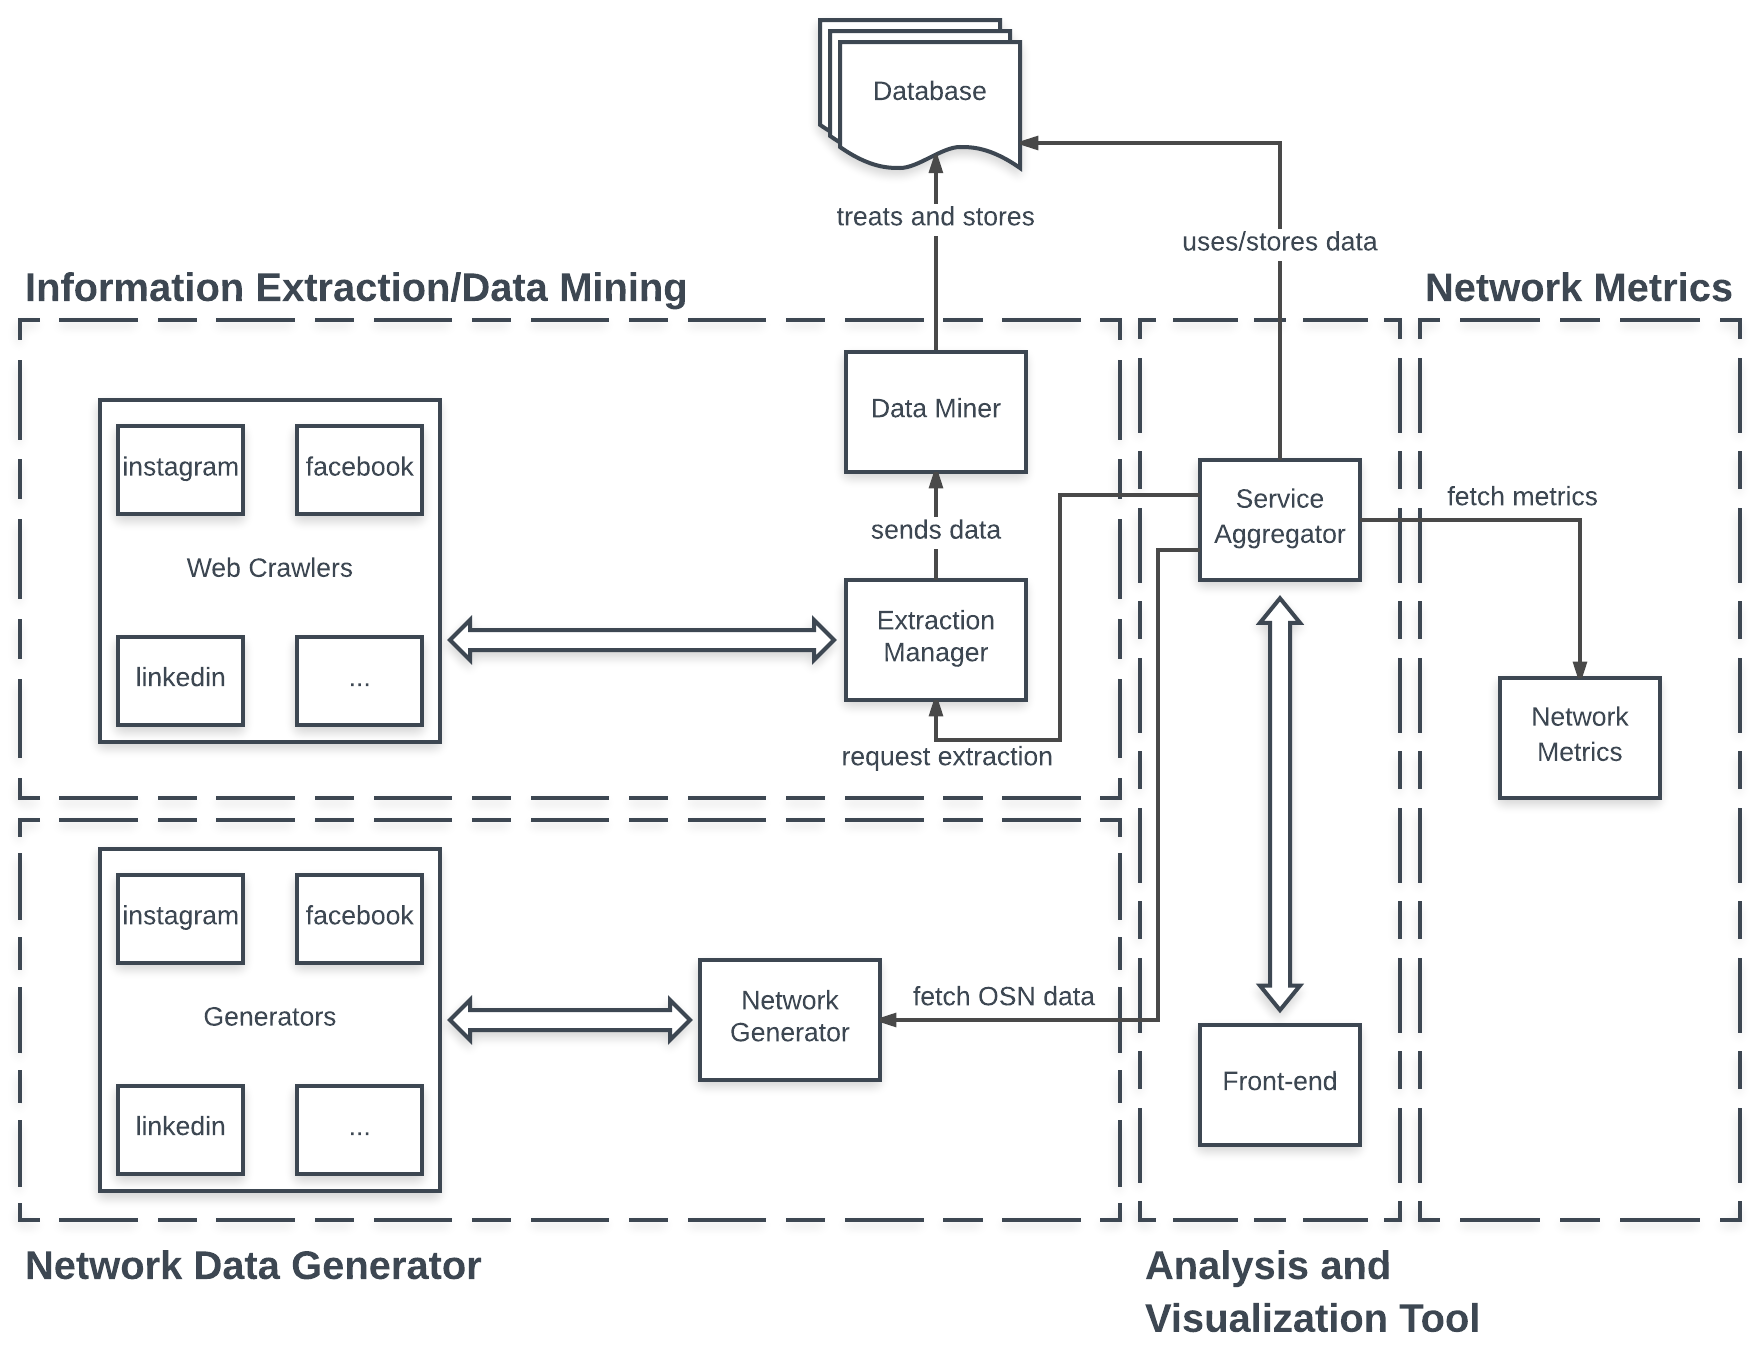
\includegraphics[width=1.2\textwidth]{img/architecture_v3.png}
\end{center}
\caption{\label{img:architectureprop} System architecture proposal.}
\end{figure}

\subsection{General overview}
As the interaction of the software components may be clear from the diagram, the role of each module is not clear by simple
diagram observation, an underlying explanation of each component is needed in order to understand the system.\\
\indent We will follow a \textit{top down} approach for explaining the system architecture. First let us be clear about the two
main and distinct parts of the system:
\begin{itemize}
    \item \textbf{\textit{Information extraction and data mining}} - All the other components are built for extracting information
    from existent databases, or from \glspl{osn} (through the \textbf{Web Crawler}) and store information being information properly treated before stored;
    \item \textbf{\textit{Network Data Generator}} - For sake of a ease of development process, and also to assure a fallback strategy upon information extraction failure, we create a network generator module that basically generates data models confined to the data schemas that we previously presented for Facebook and LinkedIn;
    \item \textbf{\textit{Network metrics}} - This module acts as a isolated component that is dedicated to perform calculations and algorithms on stored networks. It will feed metrics as requests by other components;
    \item \textbf{\textit{Analysis and Application/Visualization}} - The tool that directly interacts with the end user is composed by a \textbf{Service Aggregator} that fetches data from a database, requests extractions to the application back-end and runs calculations and algorithms on top of stored networks as the user requests by interacting with a \textbf{Front-end} that provides the visualization and interaction features.
\end{itemize}

\subsection{Detailed Components Description}
The components presented in Figure \ref{img:architectureprop} more detailed explanation, next we look more carefully into each on of the components.
\begin{itemize}
    \item \textbf{\textit{\acrfull{osn}}} - This are the object of study, the source of information that the systems will process and analyze;
    \item \textbf{\textit{Web Crawler}} - The \textbf{Web Crawler} consists in a set of modules for crawling each one of the \glspl{osn} (\textit{fb-extraction} and other modules);
    \item \textbf{\textit{Extraction Manager}} - This module consists in a wrapper for extracting information from social networks, and allows extraction orchestration spreading extraction processes along multiple hosts, so that we can mitigate the slowness of web crawlers and extraction process in general;
    \item \textbf{\textit{Data Miner}} - The data mining process assures that we store a well defined data schema that describes in the more simplified way the state of the networks;
    \item \textbf{\textit{Database}} - The database is where we store our data. It is not represented by the \textit{classical cilindro} because it resembles relational databases, and the possibility of using non relational databases such as document databases, grows strongly within the project, and the reason is the unstructured data that we will be storing into our database. We also plan on feeding some data through already existing databases, instead of crawling data from \gls{osn}. This databases may be provided from projects that we already mentioned in this document  (\hyperref[sec:otherdatasources]{Section 3.3.6}), such as \cite{kunegis2013konect}. This data would be accessed through the \textbf{Data Miner}, or a new module could be constructed exclusively to feed this data to our database;
    \item \textbf{\textit{Generator}} - a generator is a simple module that creates contextualized sets of data in order to fed our front end with the expected data that would come from the extraction module;
    \item \textbf{\textit{Network metrics}} - These module fetches data directly from the database in order to perform network operations that may be heavy. Isolating this component will allow logic separation from the service aggregator and will allow a separated infrastructure deploy, so that we may have dedicated computer resources on network metrics calculations;
    \item \textbf{\textit{Service Aggregator}} - Ideally this component application will read the already normalized information from the database, run \glspl{sna} calculations and algorithms against the stored networks, and request data to the back-end (the Information extraction and data mining super component). The Service aggregator is also responsible for communicating with network measures component in order to fetch metrics about a given network as the user requests to access it;
    \item \textbf{\textit{Front-end}} - The front-end will render the networks to the user, and will allow the user to interact with the network; these interactions will be defined in the requirements specifications.
\end{itemize}
